\documentclass[tikz,border=8pt]{standalone}
\usepackage{amsmath}
\usetikzlibrary{arrows.meta,positioning,fit,calc}

\begin{document}
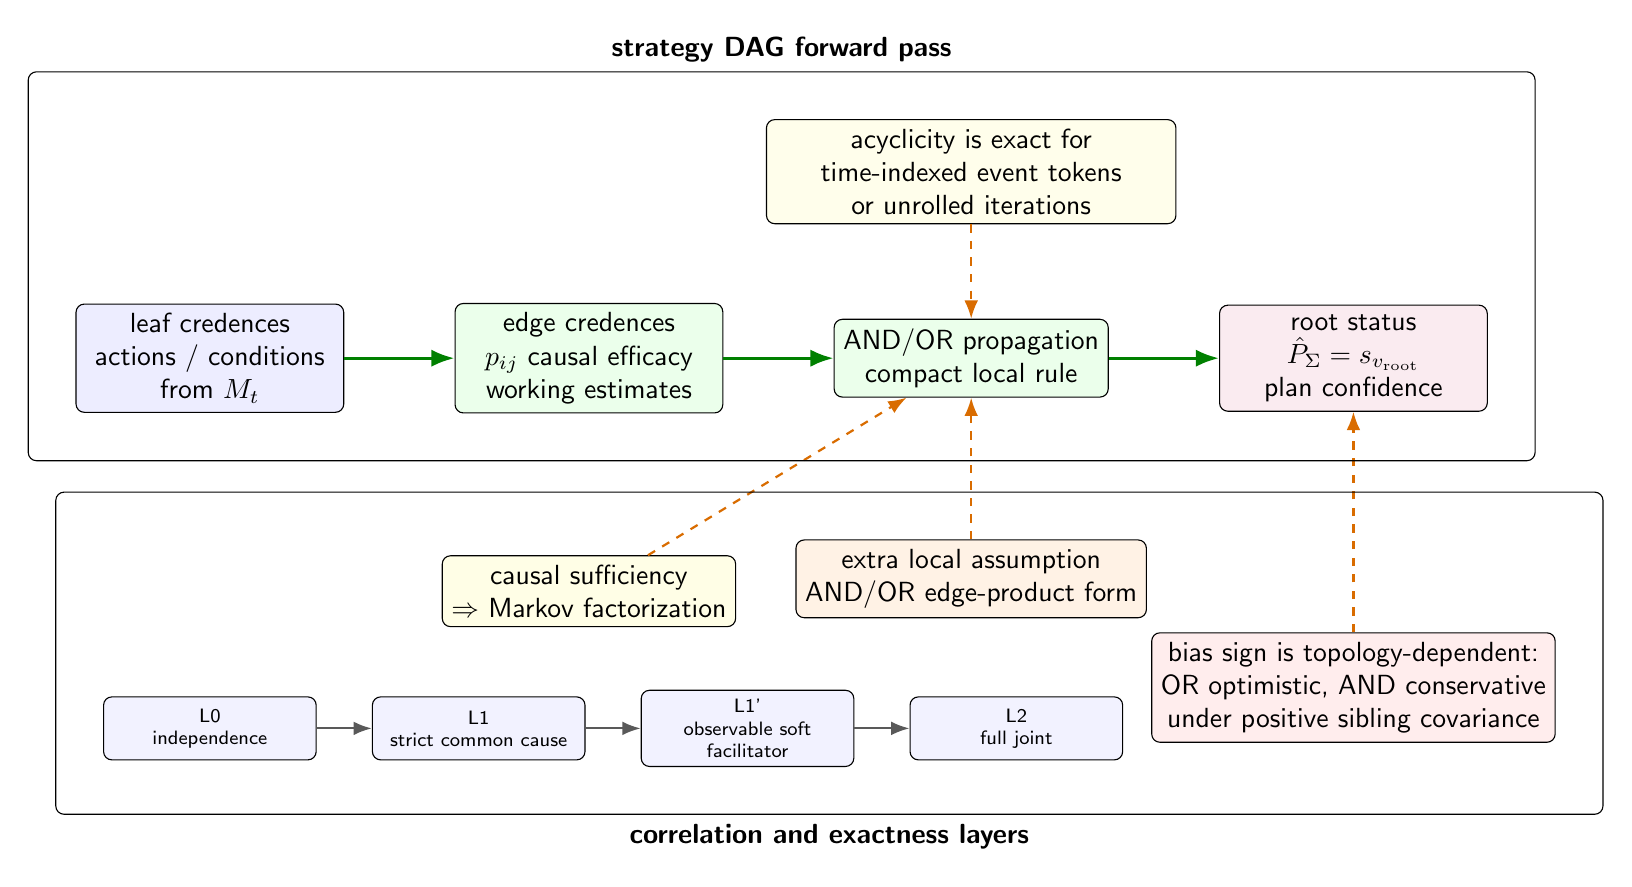
\begin{tikzpicture}[
  font=\sffamily,
  box/.style={draw, rounded corners=3pt, align=center, minimum width=34mm, minimum height=9mm, fill=white},
  small/.style={draw, rounded corners=3pt, align=center, minimum width=27mm, minimum height=8mm, fill=white, font=\sffamily\scriptsize},
  arrow/.style={-Latex, thick, draw=black!65},
  good/.style={-Latex, very thick, draw=green!50!black},
  warn/.style={-Latex, thick, dashed, draw=orange!85!black},
  note/.style={align=center, font=\sffamily\scriptsize}
]

\node[box, fill=blue!7] (leaves) {leaf credences\\actions / conditions\\from $M_t$};
\node[box, right=14mm of leaves, fill=green!8] (edges) {edge credences\\$p_{ij}$ causal efficacy\\working estimates};
\node[box, right=14mm of edges, fill=green!8] (combine) {AND/OR propagation\\compact local rule};
\node[box, right=14mm of combine, fill=purple!8] (root) {root status\\$\hat P_\Sigma=s_{v_{\rm root}}$\\plan confidence};

\draw[good] (leaves) -- (edges);
\draw[good] (edges) -- (combine);
\draw[good] (combine) -- (root);

\node[box, below=18mm of edges, fill=yellow!10] (cmc)
  {causal sufficiency\\$\Rightarrow$ Markov factorization};
\node[box, below=18mm of combine, fill=orange!10] (local)
  {extra local assumption\\AND/OR edge-product form};
\draw[warn] (cmc) -- (combine);
\draw[warn] (local) -- (combine);

\node[small, below=36mm of leaves, fill=blue!5] (l0) {L0\\independence};
\node[small, right=7mm of l0, fill=blue!5] (l1) {L1\\strict common cause};
\node[small, right=7mm of l1, fill=blue!5] (l1p) {L1'\\observable soft\\facilitator};
\node[small, right=7mm of l1p, fill=blue!5] (l2) {L2\\full joint};
\draw[arrow] (l0) -- (l1);
\draw[arrow] (l1) -- (l1p);
\draw[arrow] (l1p) -- (l2);

\node[box, below=28mm of root, fill=red!7, minimum width=44mm] (bias)
  {bias sign is topology-dependent:\\OR optimistic, AND conservative\\under positive sibling covariance};
\draw[warn] (bias) -- (root);

\node[box, above=12mm of combine, fill=yellow!8, minimum width=52mm] (time)
  {acyclicity is exact for\\time-indexed event tokens\\or unrolled iterations};
\draw[warn] (time) -- (combine);

\node[draw, rounded corners=3pt, fit=(leaves)(edges)(combine)(root)(time), inner sep=6mm,
  label={[font=\sffamily\bfseries]above:strategy DAG forward pass}] {};
\node[draw, rounded corners=3pt, fit=(cmc)(local)(l0)(l1)(l1p)(l2)(bias), inner sep=6mm,
  label={[font=\sffamily\bfseries]below:correlation and exactness layers}] {};

\end{tikzpicture}
\end{document}
